%# -*- coding: utf-8-unix -*-
%%==================================================
\chapter{哈夫曼树}
\label{chap3}

\begin{itemize}[noitemsep,topsep=0pt,parsep=0pt,partopsep=0pt]
	\item 知识点:讲解相关知识点。
	\item 题型:直接上真题。
\end{itemize}

\section{知识点和方法论}

\subsection{知识点}
\begin{itemize}[noitemsep,topsep=0pt,parsep=0pt,partopsep=0pt]
	\item 带权路径长度计算$$ WPL = \sum \mbox{节点的值} * \mbox{到这个节点的边的条数} $$
\end{itemize}


\subsection{方法论}
\begin{itemize}[noitemsep,topsep=0pt,parsep=0pt,partopsep=0pt]
	\item 左小右大(虽然不一定要这么做)
	\item 左0右1
\end{itemize}


\section{真题实战}


\subsection{2015年}

\begin{lstlisting}[basicstyle=\small\ttfamily, caption={}, numbers=none]
给定集合{15 , 3 , 14, 2 , 6 , 9, 16,17}
1) 用矩形表示外部结点,用圆圈表示内部节点,构造相应的哈夫曼树;
2) 算带权路径长度;
3) 写出哈夫曼编码;
\end{lstlisting}
~\\
解:\newline
\begin{figure}[H]
	\centering  % 环境中的内容居中排版
	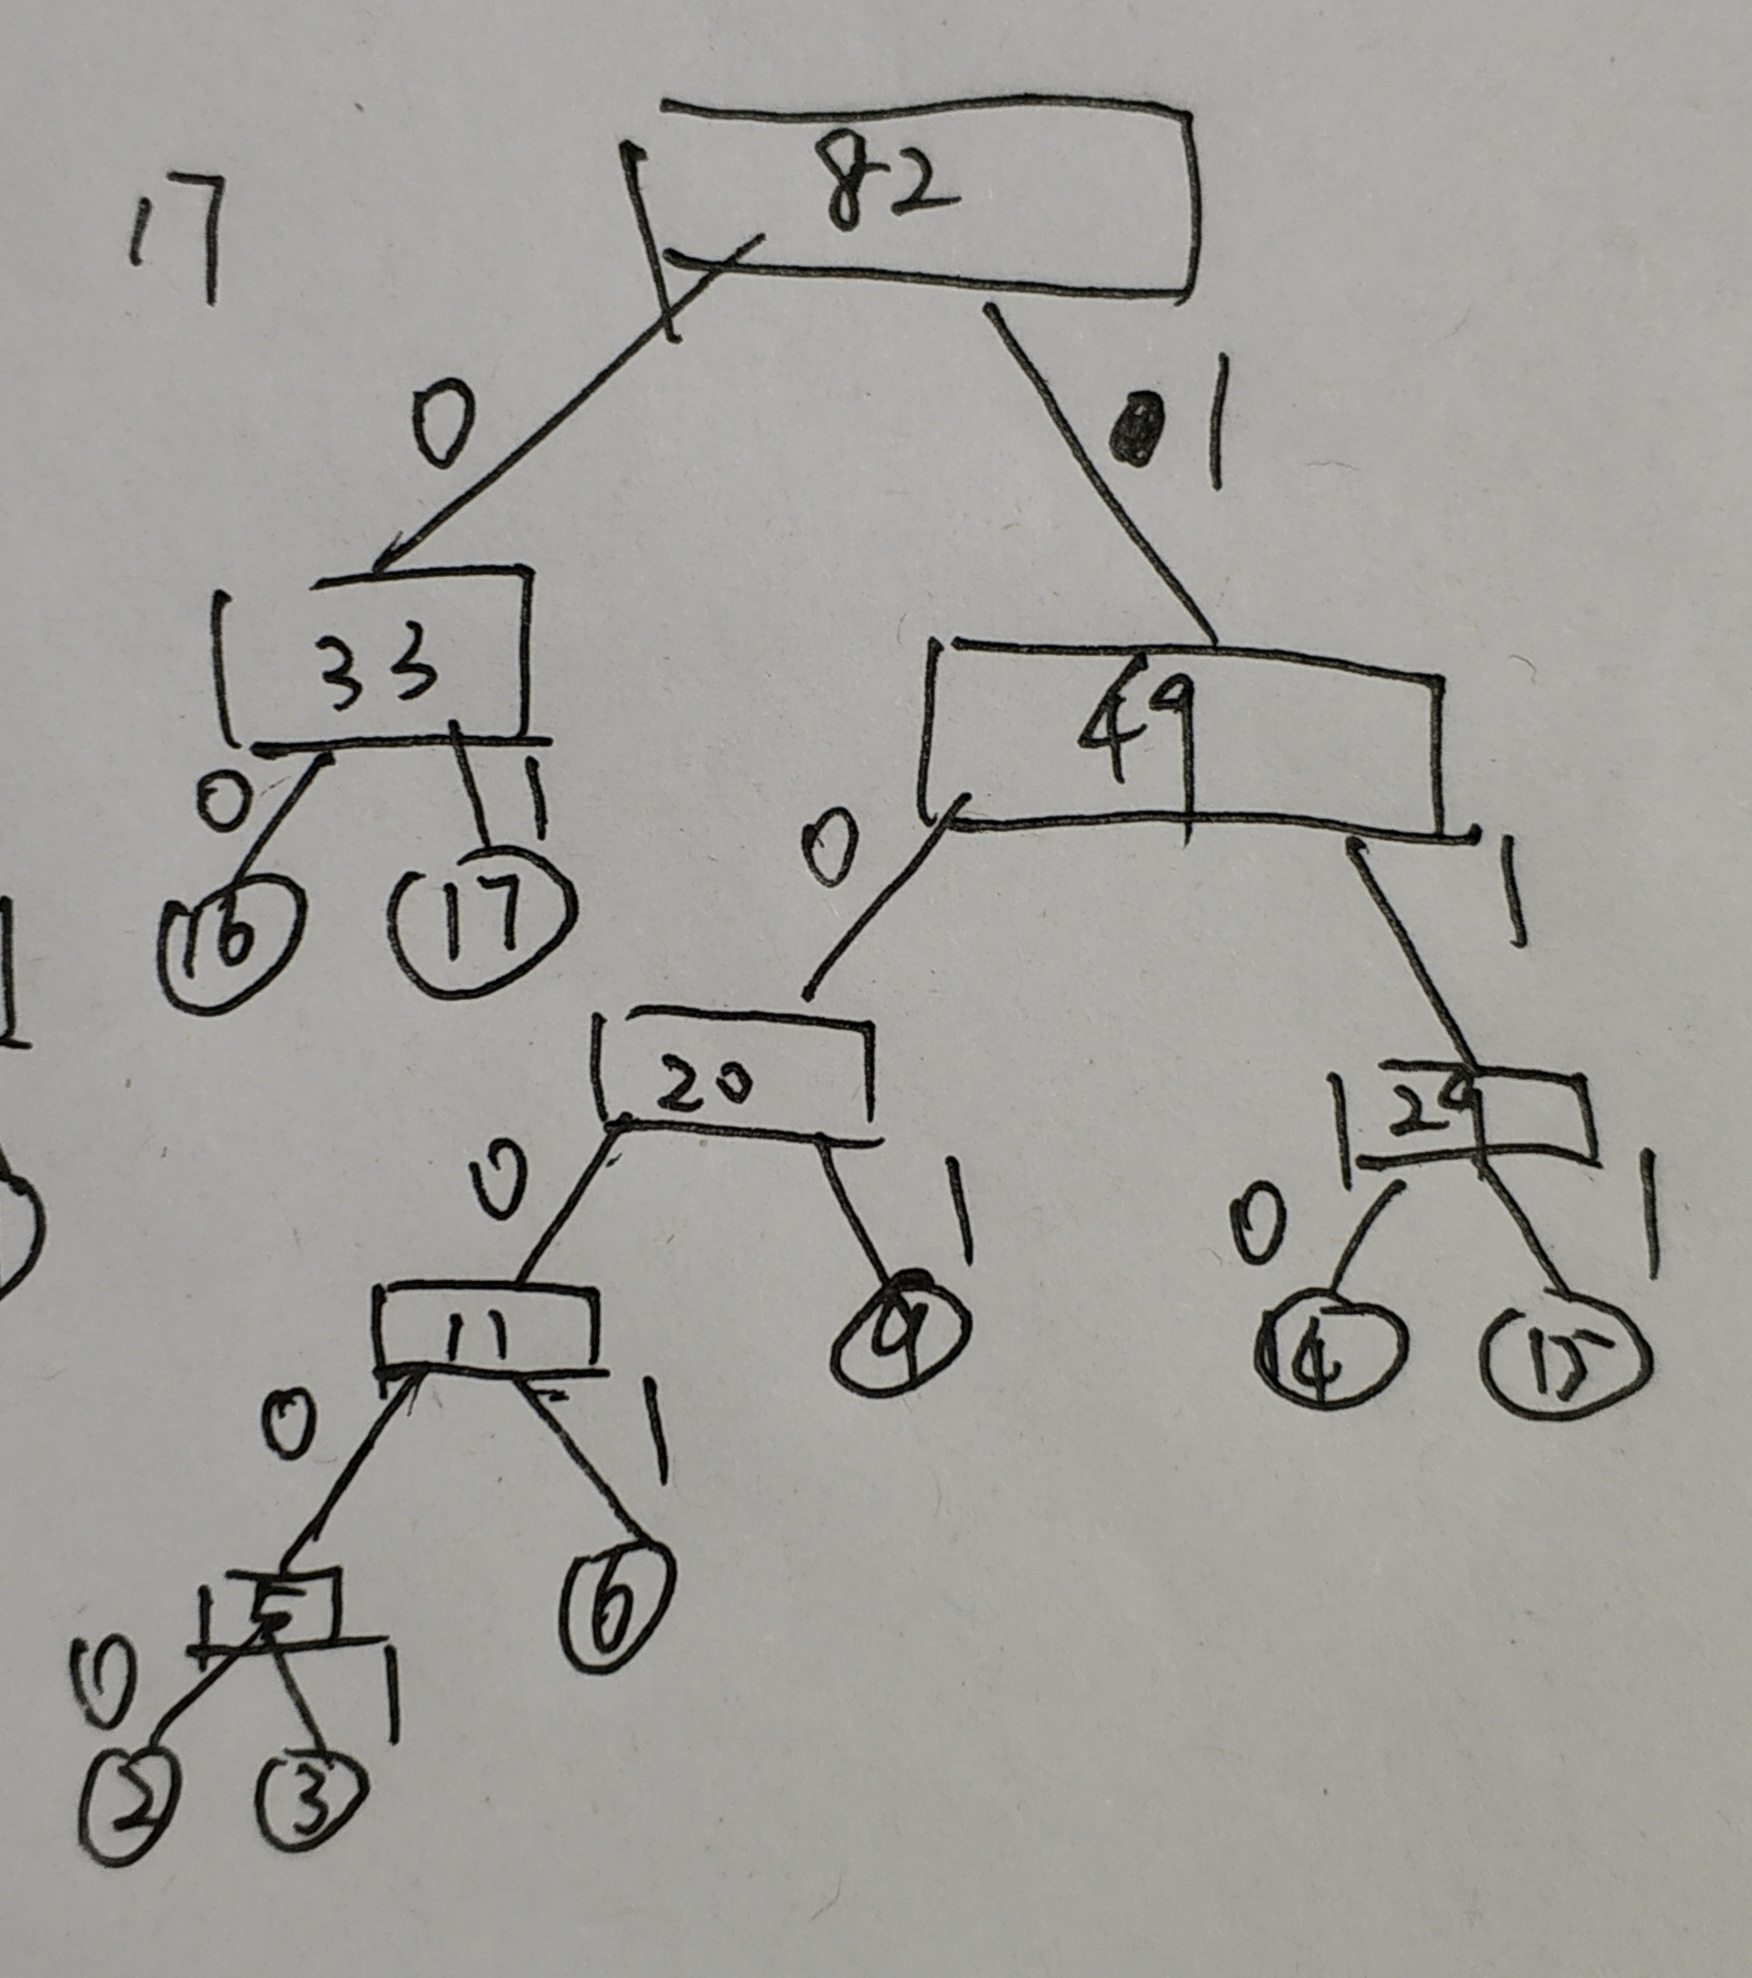
\includegraphics[scale=0.3]{example/chapter3/IMG_20181127_210022.png}
\end{figure}

2)\newline
$$ WPL =  16 * 2 + 17 * 2 + 14 *3 + 15 * 3 + 9 *3 + 6 * 4 + (2+3)* 5 = 229 $$
3)\newline
15:111\newline
14:110\newline
9:101\newline
6:1001\newline
2:10000\newline
3:10001\newline
16:00\newline
17:01\newline


\subsection{2017年}
\begin{figure}[H]
	\centering  % 环境中的内容居中排版
	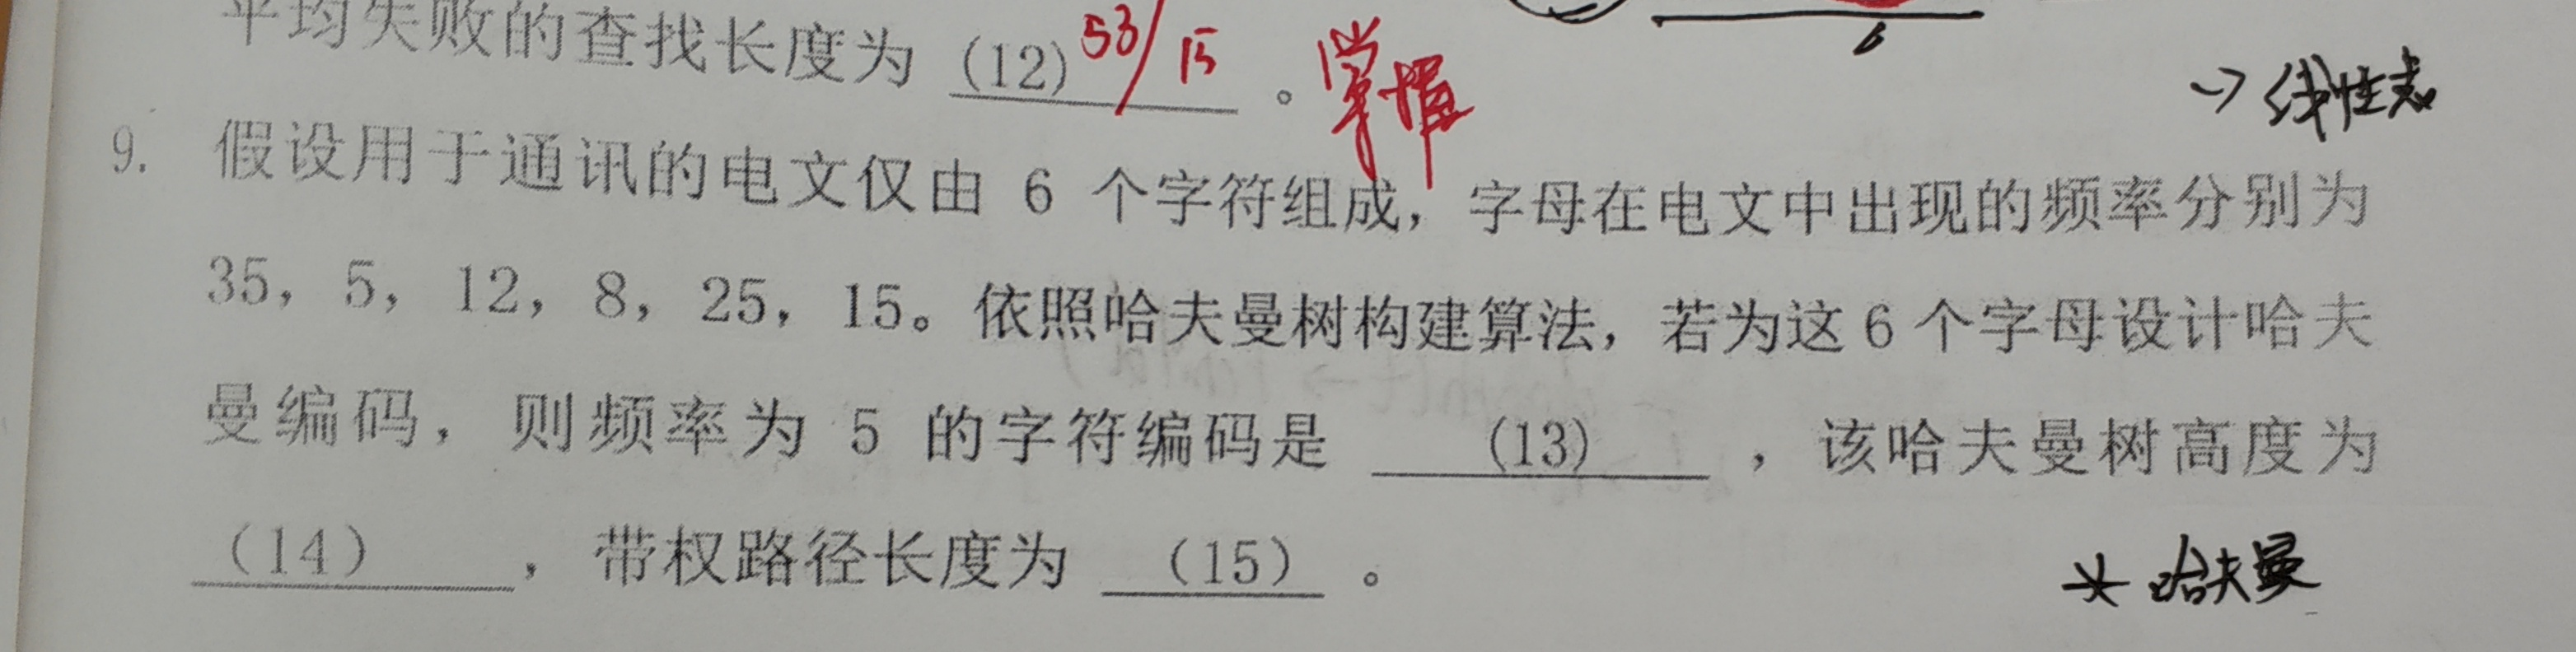
\includegraphics[scale=0.1]{example/chapter3/IMG_20181128_111603.png}
\end{figure}

解:\newline

\begin{figure}[H]
	\centering  % 环境中的内容居中排版
	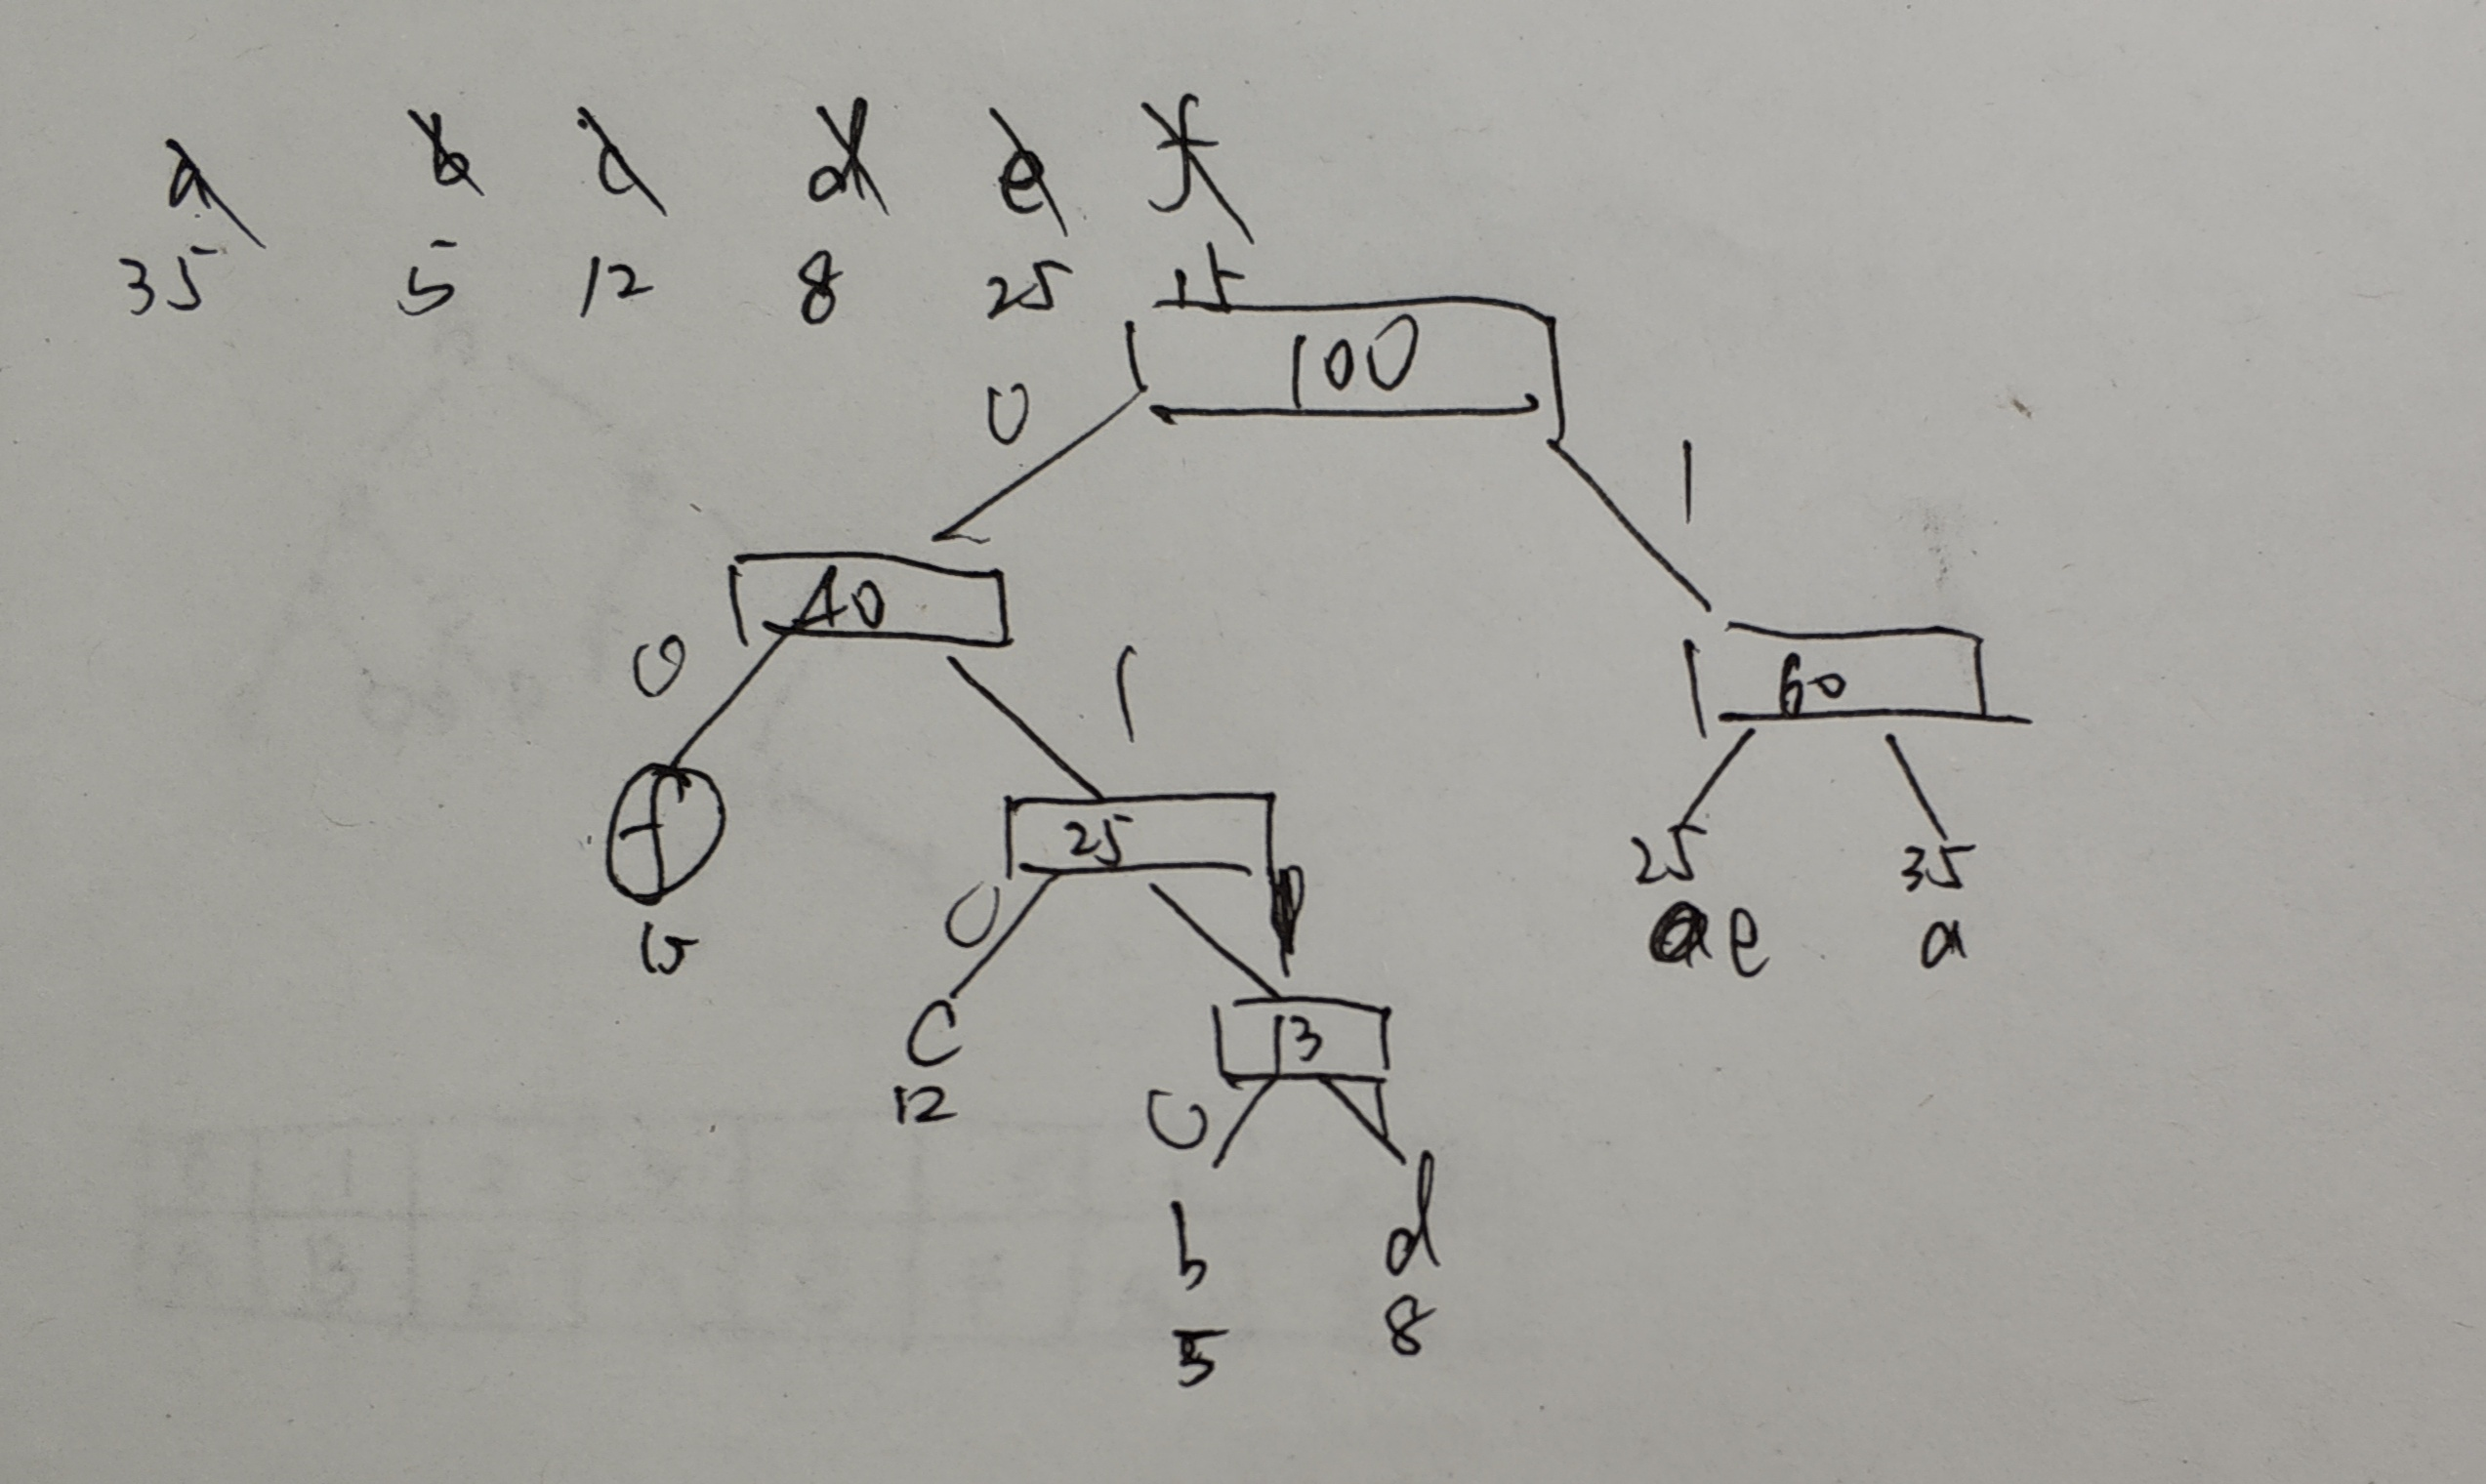
\includegraphics[scale=0.1]{example/chapter3/IMG_20181128_112049.png}
\end{figure}
~\\
5的编码 0110(不唯一,最好遵守左小右大,左0右1)\newline
高度   5\newline
$$WPL = (5*4 +8*4 + 12*3 + 15 *2 + 25 * 2 + 35 *2)=238 $$